\chapter{This is introduction}\label{ch:introduction}

\ldots

\instructionsintroduction


% Some dummy code to make sure bibtex does not complain.
Illustration of how to include citations \cite{Meert2011PhD} and \cite{VandenBroeck2011IJCAI}. Lorem ipsum dolor sit amet, consetetur sadipscing elitr, sed diam nonumy eirmod tempor invidunt ut labore et dolore magna aliquyam erat, sed diam voluptua. At vero eos et accusam et justo duo dolores et ea rebum. Stet clita kasd gubergren, no sea takimata sanctus est Lorem ipsum dolor sit amet.

And yet another citation \cite{FrRo2010Diffusion}.

% Some dummy code to get at least 1 entry in the nomenclature.
Introducing some symbol: $\Theta$.
\nomenclature{$\Theta$}{A nice symbol}

% Some dummy code to get at least 1 entry in the list of
% abbreviations.
\glossary{name=MD,description=molecular dynamics}

% Some dummy code show how to include images.
\begin{figure}
  \centering
  \medskip
  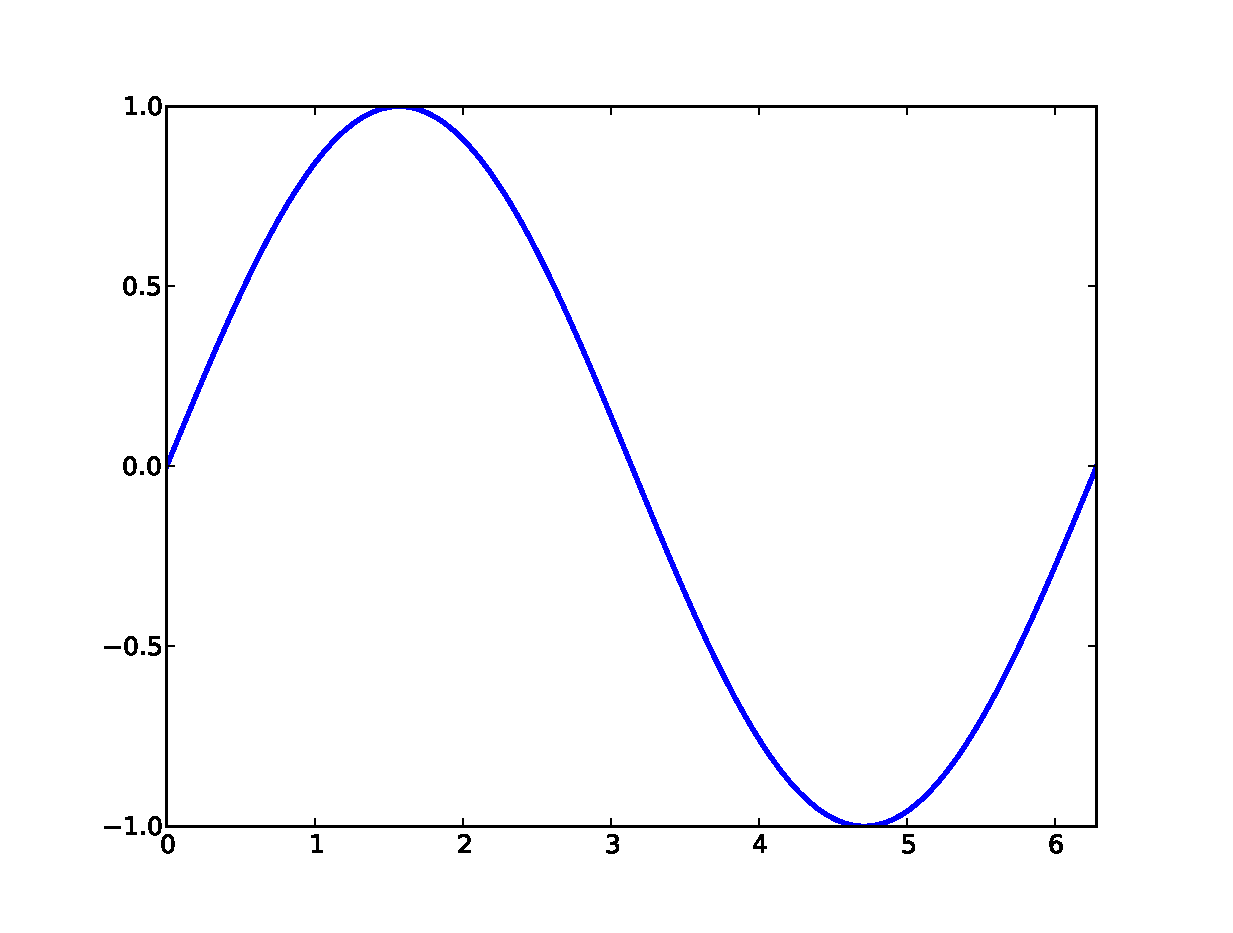
\includegraphics[width=.9\textwidth]{sine}
  \caption{Illustration of how to include a figure. }
  \label{fig:sine}
\end{figure}





%%%%%%%%%%%%%%%%%%%%%%%%%%%%%%%%%%%%%%%%%%%%%%%%%%
% Keep the following \cleardoublepage at the end of this file, 
% otherwise \includeonly includes empty pages.
\cleardoublepage

% vim: tw=70 nocindent expandtab foldmethod=marker foldmarker={{{}{,}{}}}
